%%%%%%%%%%%%%%%%%%%%%%%%%%%%%%%%%%%%%%%%%
% Beamer Presentation
% LaTeX Template
% Version 1.0 (10/11/12)
%
% This template has been downloaded from:
% http://www.LaTeXTemplates.com
%
% License:
% CC BY-NC-SA 3.0 (http://creativecommons.org/licenses/by-nc-sa/3.0/)
%
%%%%%%%%%%%%%%%%%%%%%%%%%%%%%%%%%%%%%%%%%

%----------------------------------------------------------------------------------------
%	PACKAGES AND THEMES
%----------------------------------------------------------------------------------------

\documentclass{beamer}

\mode<presentation> {

% The Beamer class comes with a number of default slide themes
% which change the colors and layouts of slides. Below this is a list
% of all the themes, uncomment each in turn to see what they look like.

%\usetheme{default}
%\usetheme{AnnArbor}
%\usetheme{Antibes}
%\usetheme{Bergen}
%\usetheme{Berkeley}
\usetheme{Berlin}
%\usetheme{Boadilla}
%\usetheme{CambridgeUS}
%\usetheme{Copenhagen}
%\usetheme{Darmstadt}
%\usetheme{Dresden}
%\usetheme{Frankfurt}
%\usetheme{Goettingen}
%\usetheme{Hannover}
%\usetheme{Ilmenau}
%\usetheme{JuanLesPins}
%\usetheme{Luebeck}
%\usetheme{Madrid}
%\usetheme{Malmoe}
%\usetheme{Marburg}
%\usetheme{Montpellier}
%\usetheme{PaloAlto}
%\usetheme{Pittsburgh}
%\usetheme{Rochester}
%\usetheme{Singapore}
%\usetheme{Szeged}
%\usetheme{Warsaw}

% As well as themes, the Beamer class has a number of color themes
% for any slide theme. Uncomment each of these in turn to see how it
% changes the colors of your current slide theme.

%\usecolortheme{albatross}
%\usecolortheme{beaver}
%\usecolortheme{beetle}
%\usecolortheme{crane}
%\usecolortheme{dolphin}
%\usecolortheme{dove}
%\usecolortheme{fly}
%\usecolortheme{lily}
%\usecolortheme{orchid}
%\usecolortheme{rose}
%\usecolortheme{seagull}
%\usecolortheme{seahorse}
%\usecolortheme{whale}
%\usecolortheme{wolverine}

%\setbeamertemplate{footline} % To remove the footer line in all slides uncomment this line
\setbeamertemplate{footline}[page number] % To replace the footer line in all slides with a simple slide count uncomment this line

\setbeamertemplate{navigation symbols}{} % To remove the navigation symbols from the bottom of all slides uncomment this line
}

\usepackage{graphicx} % Allows including images
\usepackage{booktabs} % Allows the use of \toprule, \midrule and \bottomrule in tables
\usepackage{pgfplots}
\pgfplotsset{compat=1.16}
\usepgfplotslibrary{statistics}
%----------------------------------------------------------------------------------------
%	TITLE PAGE
%----------------------------------------------------------------------------------------

\title[Short title]{How useful are corpus-based methods for extrapolating psycholinguistic variables? Mandera et al. (2015)} % The short title appears at the bottom of every slide, the full title is only on the title page

\author{Shawon Ashraf} % Your name
\institute[IMS] % Your institution as it will appear on the bottom of every slide, may be shorthand to save space
{
Universität Stuttgart \\ % Your institution for the title page % Your email address
}
\date{January 18, 2022} % Date, can be changed to a custom date

\begin{document}

\begin{frame}
\titlepage % Print the title page as the first slide
\end{frame}

%\begin{frame}
%\frametitle{Overview} % Table of contents slide, comment this block out to remove it
%\tableofcontents % Throughout your presentation, if you choose to use \section{} and \subsection{} commands, these will automatically be printed on this slide as an overview of your presentation
%\end{frame}

%----------------------------------------------------------------------------------------
%	PRESENTATION SLIDES
%----------------------------------------------------------------------------------------

%------------------------------------------------
\section{Introduction} % Sections can be created in order to organize your presentation into discrete blocks, all sections and subsections are automatically printed in the table of contents as an overview of the talk
%------------------------------------------------

%\subsection{Before we begin} % A subsection can be created just before a set of slides with a common theme to further break down your presentation into chunks

\begin{frame}
\frametitle{Which of the following words would be more meaningful together?}
\begin{table}[]
\begin{tabular}{@{}lll@{}}
\toprule
Birthday & Cakes   & Candles \\ \midrule
Race     & Vehicle & Bicycle \\ \bottomrule
\end{tabular}
\end{table}
\end{frame}

%------------------------------------------------

\begin{frame}
\frametitle{How to know which words go together?}
\begin{itemize}
\item \textbf{Distributional Semantics:} words with similar use cases or meanings tend to be grouped together in sentences (Firth, 1950, Distributional Hypothesis).
    \begin{itemize}
        \item Given large amount of text, or corpora, statistical methods \textbf{estimate} patterns and properties in text.
    \end{itemize}
\item Finding word groups is easier for humans
    \begin{itemize}
        \item What about psycholinguistic variables? 
        \item Especially Affective Ratings, Age of Acquisition or AoA (when words are acquired) Ratings etc.
        \item \textbf{Can these "Ratings" be estimated using properties from texts?}
    \end{itemize}
\end{itemize}
\end{frame}

%-----------------------------------------------
\begin{frame}
\frametitle{Goals of the paper}
\begin{itemize}
\item Use \textbf{vectorized representation} words and their distributional properties to extrapolate ratings
\item \textbf{Correlate} the extrapolation results with real world experiment results.
\item Check if extrapolated ratings can be used in \textbf{predicting psycholinguistic variables}
\end{itemize}
\end{frame}

%------------------------------------------------

% ---------------- Methods section
\section{Methods}
\begin{frame}{Word Similarity Representation}
    \begin{itemize}
        \item Latent Semantic Analysis + Bag of Words
        \item Topic based models using Latent Dirichlet Allocation
        \item Pointwise Mutual Information (PMI)
        \item Skipgram vectors
    \end{itemize}
\end{frame}

\begin{frame}{Bag of words}
    \begin{figure}
        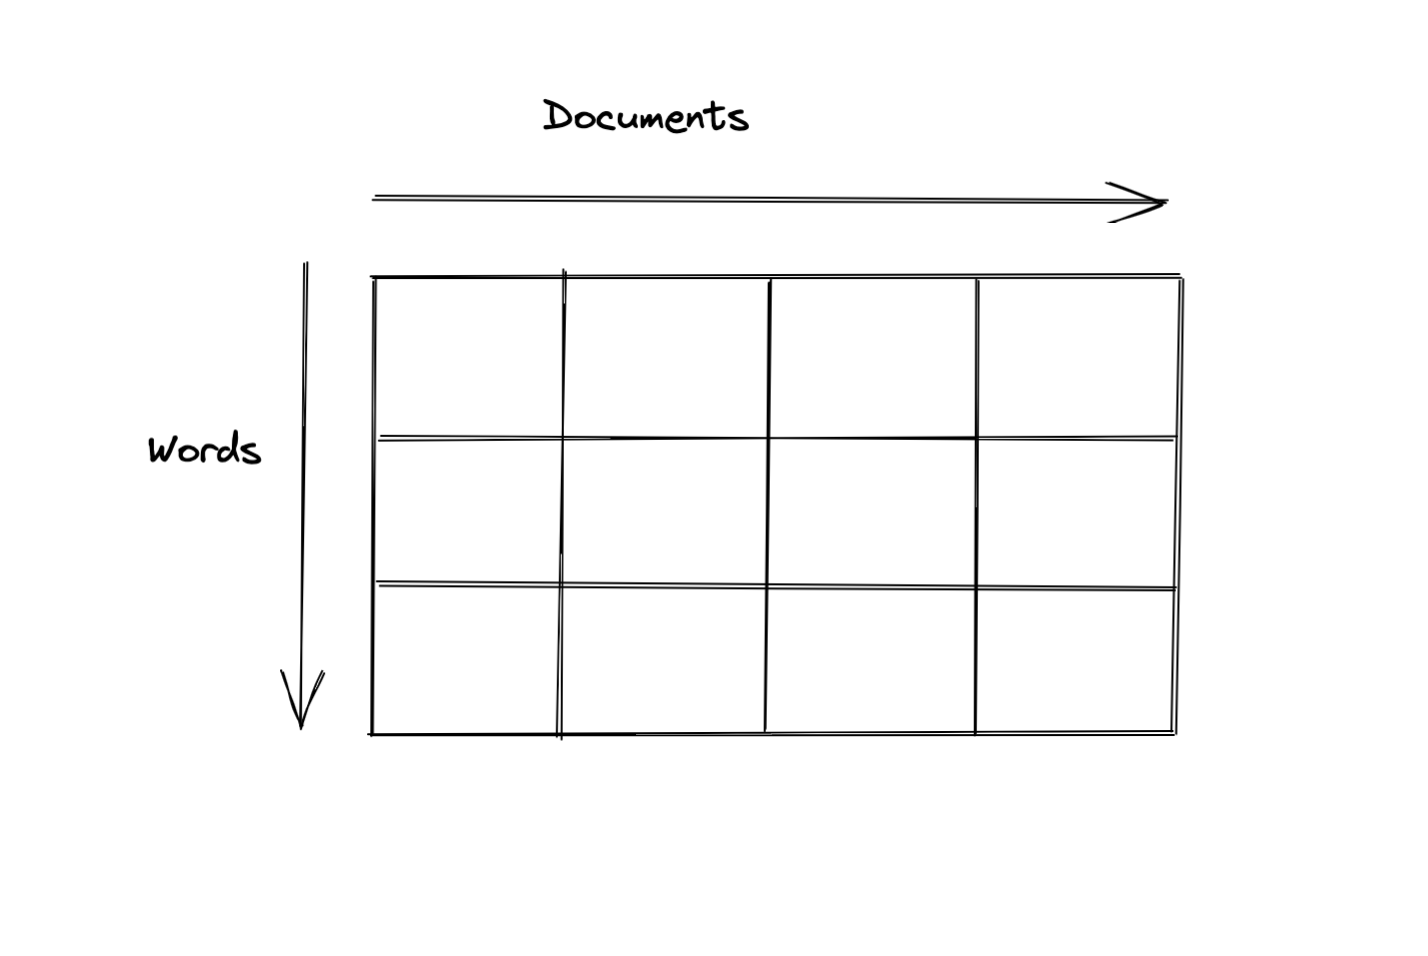
\includegraphics[width=1.0\linewidth]{bow.png}
    \end{figure}
\end{frame}

\begin{frame}{Latent Semantic Analysis (LSA)}
    \begin{itemize}
        \item Bag of Words vectors can have very large dimensions
        \item Inefficient for large vocabularies
        \item Compression is required
            \begin{itemize}
                \item Singular Value Decomposition (SVD)
            \end{itemize}
    \end{itemize}
\end{frame}

\begin{frame}
%\frametitle{Blocks of Highlighted Text}
\begin{block}{LDA and Topic Models}
Each word in a doc is generated from a probability distribution and the Topic of a word can be derived from the distribution.
\end{block}
\end{frame}

\begin{frame}{}
    \begin{block}{LDA and Topic Models}
Each word in a doc is generated from a probability distribution and the Topic of a word can be derived from the distribution.
\end{block}
\begin{block}{PMI}
Probability of a word existing given another one is already there. Example: Car chase
\end{block}
\end{frame}

\begin{frame}{}
    \begin{block}{LDA and Topic Models}
Each word in a doc is generated from a probability distribution and the Topic of a word can be derived from the distribution.
\end{block}
\begin{block}{PMI}
Probability of a word existing given another one is already there. Example: Car chase
\end{block}

\begin{block}{Skipgram}
Given a word as input estimates a certain number of neighbors of that word. Can also be used to know which words have a higher probability of being together. (Word2Vec vectors with Skipgram \cite{p1})
\end{block}
\end{frame}

% ---------------- extrapolation
\begin{frame}{Extrapolation Techniques}
\begin{block}{Random Forest}
    \begin{itemize}
        \item A collection of decision trees
        \item Each tree has a different role to learn in ensemble
        \item Knowledge of all the trees are combined together
    \end{itemize}
\end{block}

\begin{block}{k Nearest Neighbors}
    \begin{itemize}
        \item k Groups of data points
        \item Groups based on distance from a group centroid
        \item Similar words stay in the same group (based on distance)
    \end{itemize}
\end{block}
\end{frame}

% ------------- dataset
\begin{frame}{Dataset}
    \begin{itemize}
        \item English Subtitles from Open Subtitles website
            \begin{itemize}
                \item 69328 documents
                \item Lemmatized with Stanford Tagger
            \end{itemize}
        \item Ratings
            \begin{itemize}
                \item AoA
                \item Correctness
                \item Affective (valence, dominance, arousal)
            \end{itemize}
    \end{itemize}
\end{frame}

% ------------- setup
\begin{frame}{Experimental Setup}
    \begin{itemize}
        \item 25:75 $\rightarrow$ Train:Test
        \item Baselines
            \begin{itemize}
                \item Logarithmic and Semantic models which do not use word vectors
            \end{itemize}
        \item Window size of 5 for Skipgram
        \item 100 estimators in the random forest model
    \end{itemize}
\end{frame}

\section{Results}
\begin{frame}{Results}
\begin{itemize}
    \item For all variable ratings kNN is the best performing model
    \item Random Forest results are close to kNN
    \item Especially for correctness and affective ratings, the baseline performance is poor
\end{itemize}
\end{frame}

\begin{frame}{Results}
\begin{itemize}
    \item However kNN and Random Forest suffer in affective rating extrapolation
    \item Best correlation score being 0.694 whereas for correctness and AoA they score well above 0.720
\end{itemize}
\end{frame}

\begin{frame}{Results}
\begin{itemize}
    \item Extrapolated ratings show significant variance from the actual ratings
    \begin{itemize}
        \item Ratings were compared against BLP, ELP ratings
        \item Especially in affective ratings (0.67 in Valence against BLP)
    \end{itemize}
    \item Authors suspect artefacts in the extrapolation procedure
\end{itemize}
\end{frame}

\begin{frame}{Results}
\begin{itemize}
    \item Dichotomization and Binning for AoA
    \begin{itemize}
        \item \textbf{Dichotomization:} If extrapolated ratings were used in another task how precise the results will be
        \item \textbf{Binning:} Precision of finding a given set of words in the next extrapolation phase 
    \end{itemize}
    \item \textbf{Authors opine that extrapolated ratings may not be useful for accurate AoA prediction}
\end{itemize}
\end{frame}

%------------------------------------------------


%------------------------------------------------
\section{Conclusion}
%------------------------------------------------
\begin{frame}{Summary}
    \begin{itemize}
        \item Distributional features can be used to extrapolate psycholinguistic variable ratings
        \item kNN and Random Forest with vector based word representations perform better
        \item However there was no concrete answer to the original goal
    \end{itemize}
\end{frame}

\begin{frame}{Critical Reflection}
    \begin{itemize}
        \item Motivation for the corpus
        \item Why kNN and Random Forest
        \item Features for kNN and Random Forest
        \item Test set being larger than the Train set
        \item Dimension of the skipgram vectors
        \item Motivation for the Baseline models
        \item Precise definition of Correlation
        \item Why only AoA for dichotomization and binning
        \item Artefacts
    \end{itemize}
\end{frame}

\section{Questions}
\begin{frame}{Question 1}
    \begin{itemize}
        \item  The author mentioned that “ Our analyses clearly show that reporting the correlation between the original and the extrapolated variables is not sufficient to evaluate their usefulness.” Do you think this is due to the experimental design ?
    \end{itemize}
\end{frame}

\begin{frame}{Question 2}
    \begin{itemize}
        \item The order of the correlations the variables have with the original ratings are quite robust (e.g. arousal always has the lowest correlation). What could be an explanation for this?
    \end{itemize}
\end{frame}

\begin{frame}{Question 3}
    \begin{itemize}
        \item Do you think there is some fundamental problem with extrapolating ratings? Or could good enough embeddings eventually allow the extrapolations to match human judgements?
    \end{itemize}
\end{frame}


%------------------------------------------------
\section{Wrap up}
\begin{frame}
\frametitle{References}
\footnotesize{
\begin{thebibliography}{99} % Beamer does not support BibTeX so references must be inserted manually as below
\bibitem[Mikolov et al., 2013]{p1} Mikolov, Tomas and Chen, Kai and Corrado, Greg and Dean, Jeffrey (2013)
\newblock Efficient estimation of word representations in vector space
\newblock \emph{arXiv preprint arXiv:1301.3781}
\end{thebibliography}
}
\end{frame}

%------------------------------------------------

\begin{frame}
\Huge{\centerline{Thank you!}}
\end{frame}

%----------------------------------------------------------------------------------------

\end{document} 